Korzystając z~wiedzy i~doświadczeń wyniesionych z~sekcji~\ref{sec:przeglad} niniejszego sprawozdania, zdecydowaliśmy się na stworzenie systemu odpowiadającego na pytania ogólne, z~wyszczególnieniem pytań o~fakty dotyczące:
\begin{itemize}
	\item osób,
	\item miejsc,
	\item dat,
	\item cech wielkościowych,
	\item przedmiotów.
\end{itemize}

Bazą wiedzy systemu jest sieć WWW. Do wyszukiwania dokumentów w~sieci~WWW, wykorzystane zostały wyszukiwarki internetowe: \emph{Google\footnote{www.google.pl}}, \emph{Bing\footnote{www.bing.com}}, \emph{Yahoo\footnote{www.search.yahoo.com}} oraz \emph{DuckDuckGo\footnote{duckduckgo.com}}. Dodatkowo wprowadzona została opcja \emph{combined}, która zwraca rezultaty uzyskane ze wszystkich wymienionych wyżej stron. Zapytanie do wyszukiwarki jest tworzone za pomocą jednej z trzech strategii: \emph{singleQuery}, \emph{stopwords} lub \emph{chunks}. Pierwsza polega na bezpośrednim wyszukaniu wpisanego pytania, druga usuwa wyrazy ze Stop-listy przed rozpoczęciem wyszukiwania, ostatnia tworzy wiele zapytań poprzez podział zapytania na kawałki, tzw. \emph{chunks}. Podobnie jak we wcześniej omawianym systemie AskMSR~\cite{brill2002analysis}, do dalszej analizy przekazywane są jedynie \emph{snippety}, co pozwoliło na uproszczenie etapu filtracji akapitów. 
Odpowiedzią na przedstawione pytanie, będzie prosta jedno-, dwu- lub trzywyrazowa odpowiedź typu \emph{Named-Entity} oraz adres URL, z której pochodzi dany \emph{snippet}. 


\subsection{Opis algorytmu}
Na rysunku~\ref{fig:algorithm-overview}, przedstawiony został ogólny schemat algorytmu odpowiadania na pytania.

\begin{figure}[h]
    \centering
    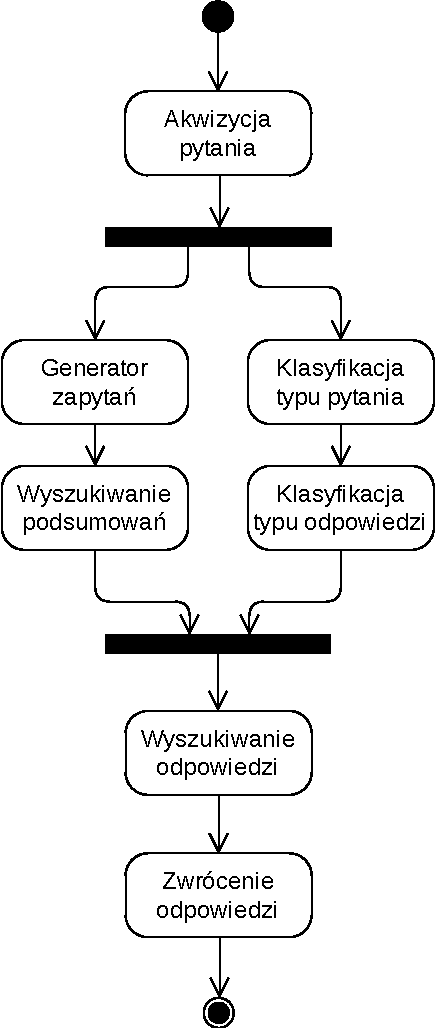
\includegraphics[width=0.7\columnwidth]{figures/WEDT-Algorytm.pdf}
    \caption{Ogólny schemat algorytmu odpowiadania na pytania}
    \label{fig:algorithm-overview}
\end{figure}

\subsubsection{Akwizycja pytania}
Pierwszym krokiem algorytmu jest akwizycja pytania od użytkownika systemu. Każde pytanie jest analizowane w~sposób indywidualny, bez przechowywania wcześniejszych pytań i~utrzymywania kontekstu. Nie zakładamy również żadnego profilowania użytkowników, ponieważ typowo proste pytania o~fakty, są ze sobą słabo powiązane. Dla każdego zapytania użytkownik wybiera strategię wyszukiwania tj. \emph{singleQuery}, \emph{stopwords} lub \emph{chunks} oraz jedną z 5 opcji wyszukiwania: \emph{Google}, \emph{Bing}, \emph{Yahoo}, \emph{DuckDuckGo} lub \emph{combined}.

\subsubsection{Klasyfikacja typu pytania i odpowiedzi}
W~kolejnym kroku następuje klasyfikacja typu pytania, a zaraz po niej określenie typu oczekiwanej odpowiedzi. Klasy pytań są definiowane przez zaimki pytające, podobnie jak w~\cite{gupta2012survey}. W naszym systemie wyróżniamy 15 rodzajów pytań. Rozpoznawane są zarówno formy podstawowe zaimków pytających, jak i formy odmienione.

Klasyfikacja typu pytania jest ściśle powiązana z pierwszym z dwóch etapów rozpoznawania typu odpowiedzi. Aby wykryć typ pytania, słowa z zapytania są kolejno sprawdzane w przygotowanym słowniku zawierającym pary typPytania-typOdpowiedzi, gdzie typPytania jest kluczem, natomiast typOdpowiedzi wartością. Słowo, które jako pierwsze będzie miało przyporządkowaną wartość w słowniku, informuje o typie pytania. Od tej reguły istnieje jeden wyjątek, który wymusza sprawdzenie kolejnych wyrazów z zapytania. Przy pytaniach \emph{Co ile ... ?}, typ pytania jest określony przez drugi wyraz posiadający odpowiednik w słowniku. Rozpoznawane pary typPytania-typOdpowiedzi przedstawiono w tabeli \todo{tabela}.

Rozpoznawanie typu odpowiedzi składa się z jednego lub dwóch etapów. Etap pierwszy odbywa się równocześnie z rozpoznawaniem typu pytania, ponieważ oczekiwanym typem odpowiedzi jest odnaleziona w słowniku wartość. Może być ona jednym słowem lub listą. Pojedyncze rozpoznawane typy odpowiedzi to: OSOBA, MIEJSCE, RZECZ, WIELKOŚĆ oraz DATA. 

Niestety nie wszystkie typy pytań jednoznacznie określają oczekiwany typ odpowiedzi, dlatego niezbędne okazało się wprowadzenie drugiego etapu. Pytania \emph{Jak?}, \emph{Jaki/Jaka/Jakie?}, oraz \emph{Który/Która/Które?} są nietrywialne, ponieważ nie można jednoznacznie przyporządkować typu oczekiwanej odpowiedzi (\emph{complex}) bez dodatkowej analizy zapytania. 

Dla pytań \emph{Jaki/Jaka/Jakie?} oraz \emph{Który/Która/Które?} typ oczekiwanej odpowiedzi jest określany poprzez odszukanie pierwszego rzeczownika, występującego pomiędzy zaimkiem pytającym a czasownikiem, którego odmiana zgodna jest z odmianą zaimka pytającego. W tym celu całe zapytanie wysyłane jest do usługi \emph{Spejd}, która zwraca między innymi leksemy poszczególnych wyrazów jak i tagsety zawierające informacje o części mowy, liczbie oraz odmianie przez przypadki. Leksem wyrazu, który jet odpowiednio odmienionym rzeczownikiem, analizowany jest następnie za pomocą usługi \emph{plWordNet}. Zapytanie zwraca między innymi listę domen, do których przynależy dany wyraz. Domeny z \emph{plWordNetu} konwertowane są na jedną lub więcej oczekiwanych typów odpowiedzi z listy: OSOBA, MIEJSCE, RZECZ, WIELKOŚĆ, DATA lub brak dopasowania. 

Jeżeli pomiędzy zaimkiem pytającym a czasownikiem nie występuje żaden pasujący rzeczownik, algorytm próbuje odnaleźć poprawnie odmieniony przymiotnik znajdujący się pomiędzy zaimkiem a czasownikiem. Gdy takowy występuje, oczekiwanym typem odpowiedzi jest WIELKOŚĆ. Jeżeli taki przymiotnik nie został odnaleziony, ostatnią szansą jest odnalezienie rzeczownika odmienionego zgodnie z zaimkiem pytającym znajdującym się za czasownikiem. Jeżeli zostanie on odnaleziony, to dalsze postępowanie jest analogiczne do sytuacji z rzeczownikiem znajdującym się pomiędzy zaimkiem a czasownikiem. 

Ostatnim wyróżnionym przypadkiem są pytania \emph{Który z?}. Dla takiego przypadku poszukiwany jest rzeczownik w liczbie mnogiej w dopełniaczu. 

Przy pytaniu \emph{Jak?} najpierw poszukiwany jest przymiotnik znajdujący się zaraz za zaimkiem pytającym. Jeżeli został odnaleziony, szukanym typem odpowiedzi jest WIELKOŚĆ. W przeciwnym wypadku oczekiwanym typem odpowiedzi może być zarówno WIELKOŚĆ, OSOBA, MIEJSCE czy RZECZ. 

\subsubsection{Generator zapytań}
Generator zapytań otrzymuje pytanie wprowadzone przez użytkownika wraz ze strategią generowania zapytania. Jeżeli wybrana została strategia \emph{singlequery}, rolą generatora zapytań jest jedynie przekazanie pytania do wyszukiwarki podsumowań. 


Aby zwiększyć liczbę uzyskanych podsumowań lub zmienić zakres poszukiwań zdecydowaliśmy się na wprowadzenie dwóch strategii: \emph{stopwords} i \emph{chunks}. Pierwsza z nich polega na usunięciu słów z zapytania, które znajdują się na Stop-liście. Tym samym do wyszukiwania wysłane zostanie okrojone zapytanie, pozbawione części słów, tak aby zwiększyć zakres poszukiwań, podobnie jak w~\cite{brill2002analysis}. Innym podejściem jest zastosowanie strategii \emph{chunks}, która polega na podziale zapytania przy pomocy usługi \emph{Chunker}. Umożliwia to zwiększenie rozmiaru zbioru wyszukanych \emph{snippetów}.

\subsubsection{Wyszukiwanie podsumowań}
Moduł wyszukiwania podsumowań, na podstawie przekazanego zapytania lub zapytań oraz typu silnika generuje zapytanie do odpowiedniej wyszukiwarki internetowej i zwraca odnalezione \emph{snippety}.

\subsubsection{Wyszukiwanie odpowiedzi}
\todo{dopisać dużo}
Każdy wyszukany \emph{snippet} zostanie poddany analizie morfologicznej, po której przyporządkowana zostanie mu odpowiednia ocena. W~każdym zdaniu, za pomocą taggera oraz \emph{plWordNetu} wyszukiwane będą \emph{Named-Entities}, które mogą stanowić potencjalną odpowiedź na pytanie.

\subsubsection{Zwrócenie odpowiedzi}
Ostatnim krokiem procesu będzie zwrócenie najlepszej odpowiedzi. Dodatkowo do odpowiedzi dołączony może zostać link ze źródłem, w~celu umożliwienia użytkownikowi systemu osobistej weryfikacji odpowiedzi.

\subsection{Dekompozycja systemu}
Stworzony system składa się z~kilku funkcjonalnych komponentów, z których część została przez nas zaimplementowana w całości, a przy pozostałych korzystamy z gotowych komponentów takich jak \emph{plWordNet} czy wyszukiwarki internetowe. Na rysunku \ref{fig:system-components} przedstawiony został podział na komponenty funkcjonalne, ze szczególnym wyróżnieniem relacji pomiędzy nimi.

\todo{Czy to zostaje?}
\begin{figure}[h]
	\centering
	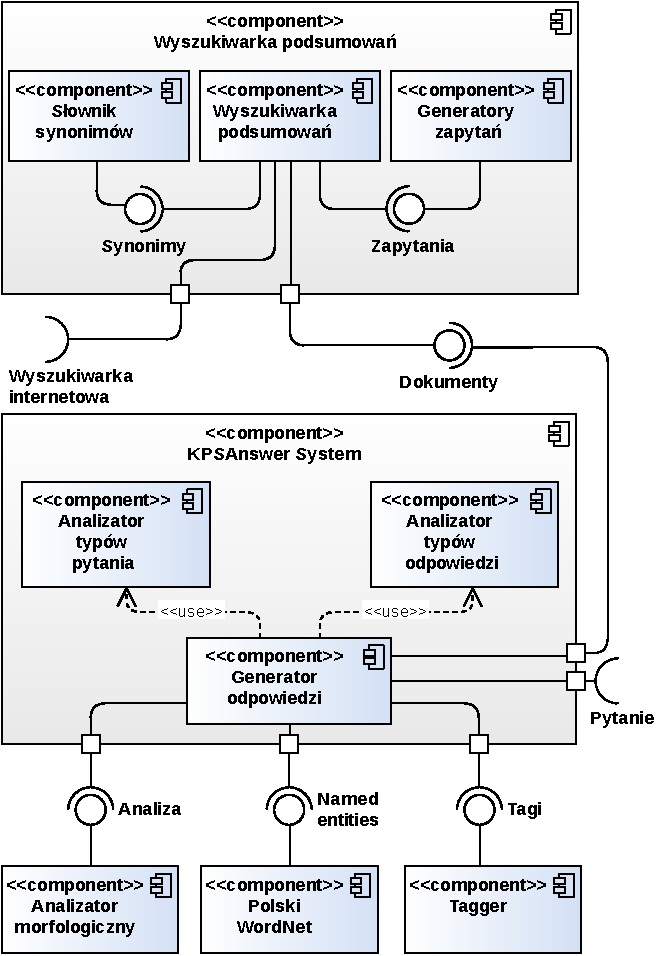
\includegraphics[width=\columnwidth]{figures/WEDT-Komponenty.pdf}
	\caption{Podział systemu KPSAnswer na funkcjonalne komponenty}
	\label{fig:system-components}
\end{figure}

System składa się z dwóch głównych komponentów:
\emph{KPS\footnote{Nazwa KPS pochodzi od pierwszych liter nazwisk autorów}} oraz wyszukiwarki podsumowań \emph{Zapytajka}, wspieranych kilkoma komponentami pobocznymi.
Komponent \emph{KPS} zajmuje się generacją odpowiedzi na pytania przychodzące z~zewnątrz, korzystając z~interfejsu \texttt{Pytania}. W~celu wygenerowania odpowiedzi, komponent ten odpytuje \emph{Zapytajkę} przy użyciu interfejsu \texttt{Dokumenty} o~zbiór podsumowań, mogących zawierać odpowiedź. \emph{Zapytajka} generuje zapytanie i zdobywa podsumowania odpytując strony implementujące interfejs \texttt{Wyszukiwarka internetowa}.


